% ថ្នាក់ទី ១១ (វិទ្យាសាស្ត្រ) · ជំពូកទី ៤ · មេរៀនទី ២ · សៀវភៅទំព័រ ១៨០–១៨៧
\chapter{ដេទែរមីណង់}

\begin{objBox}[វត្ថុបំណង]
\begin{enumerate}[1]
  \item គណនាដេទែរមីណង់លំដាប់ $2$ និងលំដាប់ $3$
  \item ដោះស្រាយប្រព័ន្ធសមីការលីនេអ៊ែរដោយប្រើដេទែរមីណង់ ។
\end{enumerate}
\end{objBox}

\section{ដេទែរមីណង់លំដាប់ 2}

កន្សោម $ad - bc$ ដែលបានពីម៉ាទ្រីស $A = \begin{bmatrix} a & b\\ c & d \end{bmatrix}$ ហៅថា ដេទែរមីណង់លំដាប់ $2$ នៃម៉ាទ្រីស $A$ ។ គេកំណត់សរសេរ $\det(A)$ ឬ $|A|$ ឬ $\begin{vmatrix} a & b\\ c & d \end{vmatrix}$ ។

\begin{formulaBox}[ដេទែរមីណង់លំដាប់ 2]
តម្លៃដេទែរមីណង់នៃម៉ាទ្រីស $A = \begin{bmatrix} a & b\\ c & d \end{bmatrix}$ គឺ $\det A = |A| = \begin{vmatrix} a & b\\ c & d \end{vmatrix} = ad - bc$ ។
\end{formulaBox}

\begin{example}[លំហាត់គំរូ ១]
គេឱ្យម៉ាទ្រីស $M = \begin{bmatrix} 2 & -3\\ 4 & 3 \end{bmatrix}$, $N = \begin{bmatrix} -4 & 14\\ 10 & 10 \end{bmatrix}$ និង $P = \begin{bmatrix} -2 & 3\\ -4 & 6 \end{bmatrix}$ ។
\begin{enumerate}[a]
  \item គណនាដេទែរមីណង់និងម៉ាទ្រីសច្រាស (បើមាន) នៃម៉ាទ្រីសនីមួយៗ ។
  \item គណនាម៉ាទ្រីស $X$ បើ $MX = N$
  \item គណនាម៉ាទ្រីស $Y$ បើ $YM = N$ ។
\end{enumerate}
\end{example}
\ans
\begin{enumerate}[a]
  \item $|M| = \begin{vmatrix} 2 & -3\\ 4 & 3 \end{vmatrix} = 6 + 12 = 18$ និង $M^{-1} = \dfrac{1}{18}\begin{bmatrix} 3 & 3\\ -4 & 2 \end{bmatrix} = \begin{bmatrix} \frac{1}{6} & \frac{1}{6}\\ -\frac{2}{9} & \frac{1}{9} \end{bmatrix}$ ។

  $|N| = \begin{vmatrix} -4 & 14\\ 10 & 10 \end{vmatrix} = (-4)(10) - 14(10) = -180$ និង $N^{-1} = -\dfrac{1}{180}\begin{bmatrix} 10 & -14\\ -10 & -4 \end{bmatrix} = \begin{bmatrix} -\frac{1}{18} & \frac{7}{90}\\ \frac{1}{18} & \frac{1}{45} \end{bmatrix}$

  $|P| = \begin{vmatrix} -2 & 3\\ -4 & 6 \end{vmatrix} = -12 + 12 = 0$, $P$ គ្មានម៉ាទ្រីសច្រាសទេ ។
  \item គេមានសមីការម៉ាទ្រីស $MX = N$ ។ បើគេគុណពីខាងឆ្វេងអង្គនីមួយៗនៃសមីការម៉ាទ្រីសនឹង $M^{-1}$ នោះគេបាន
  \[
\begin{aligned}
M^{-1}MX &= M^{-1}N \Rightarrow IX = M^{-1}N \ (\text{ព្រោះ } M^{-1}M = I)\\
&\Rightarrow X = M^{-1}N \ (\text{ព្រោះ } IX = X)
\end{aligned}
\]
  \[
\begin{gathered}
X = \frac{1}{18}\begin{bmatrix} 3 & 3\\ -4 & 2 \end{bmatrix}\begin{bmatrix} -4 & 14\\ 10 & 10 \end{bmatrix} = \frac{1}{18}\begin{bmatrix} 18 & 72\\ 36 & -36 \end{bmatrix},\\
X = \begin{bmatrix} 1 & 4\\ 2 & -2 \end{bmatrix} \text{ ។}
\end{gathered}
\]
  \item គេមានសមីការម៉ាទ្រីស $YM = N$ ។ បើគេគុណពីខាងស្តាំអង្គនីមួយៗនៃសមីការម៉ាទ្រីសនឹង $M^{-1}$ នោះគេបាន
  \[ YMM^{-1} = NM^{-1} \Rightarrow YI = NM^{-1} \Rightarrow Y = NM^{-1} \]
  \[
\begin{gathered}
Y = \begin{bmatrix} -4 & 14\\ 10 & 10 \end{bmatrix}\frac{1}{18}\begin{bmatrix} 3 & 3\\ -4 & 2 \end{bmatrix} = \frac{1}{18}\begin{bmatrix} -68 & 16\\ -10 & 50 \end{bmatrix},\\
Y = \begin{bmatrix} -\frac{34}{9} & \frac{8}{9}\\ -\frac{5}{9} & \frac{25}{9} \end{bmatrix} \text{ ។}
\end{gathered}
\]
\end{enumerate}

\begin{pro}
គេមានម៉ាទ្រីស $A = \begin{bmatrix} 3 & -1\\ 2 & 0 \end{bmatrix}$ និង $B = \begin{bmatrix} 5 & 0\\ -2 & 4 \end{bmatrix}$ ។ \quad ក. រកម៉ាទ្រីស $X$ ដែល $AX = B$ ។ \quad ខ. គណនា $(AB)^{-1}$ និង $B^{-1}A^{-1}$ រួចសន្និដ្ឋាន ។
\ans
ក. $A^{-1} = \dfrac{1}{2}\begin{bmatrix} 0 & 1\\ -2 & 3 \end{bmatrix}$, \ $X = \begin{bmatrix} -1 & 2\\ -8 & 6 \end{bmatrix}$ ។

ខ. $AB = \begin{bmatrix} 17 & -4\\ 10 & 0 \end{bmatrix}$, \ $(AB)^{-1} = \begin{bmatrix} 0 & \frac{1}{10}\\ -\frac{1}{4} & \frac{17}{40} \end{bmatrix} = B^{-1}A^{-1}$ ។
\end{pro}

\section{ដេទែរមីណង់លំដាប់ 3}

\subsection{គណនាដេទែរមីណង់លំដាប់ 3 តាមក្បួនរបស់សារុស}

គេមានដេទែរមីណង់ $\begin{vmatrix} a_1 & b_1 & c_1\\ a_2 & b_2 & c_2\\ a_3 & b_3 & c_3 \end{vmatrix}$ ។ គេអាចយកជួរទី $1$ និងទី $2$ សរសេរបន្ថែមបន្ទាប់ពីដេទែរមីណង់ ។
\begin{center}
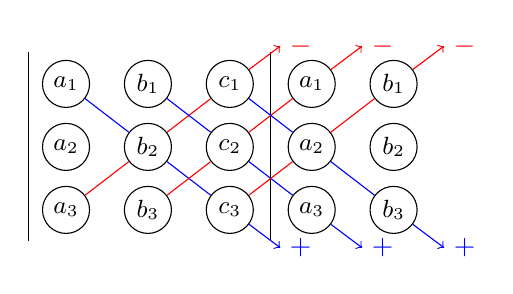
\begin{tikzpicture}[scale=0.8]
  \foreach \c/\l in {0/a,1/b,2/c,3/a,4/b} \foreach \r in {1,2,3} \node[circle,draw,inner sep=1pt,minimum size=17pt] (n\c\r) at (\c*1.3,-\r) {\small $\l_\r$};
  \draw (-0.6,-0.5) -- (-0.6,-3.5); \draw (3.25,-0.5) -- (3.25,-3.5);
  \foreach \c in {0,1,2} {\pgfmathtruncatemacro{\a}{\c+1}\pgfmathtruncatemacro{\b}{\c+2}
    \draw[->,blue] (n\c1) -- (n\a2) -- (n\b3) -- ++(0.8,-0.6) node[right] {$+$};
    \draw[->,red] (n\c3) -- (n\a2) -- (n\b1) -- ++(0.8,0.6) node[right] {$-$};}
\end{tikzpicture}
\end{center}
បន្ទាប់មកគេគណនាផលគុណនៃធាតុដែលតាមសញ្ញាព្រួញនីមួយៗ គេបាន
\begin{formulaBox}[ក្បួនសារុស]
\[
\begin{aligned}
\begin{vmatrix} a_1 & b_1 & c_1\\ a_2 & b_2 & c_2\\ a_3 & b_3 & c_3 \end{vmatrix} &= a_1b_2c_3 + b_1c_2a_3 + c_1a_2b_3\\
&\quad - a_3b_2c_1 - b_3c_2a_1 - c_3a_2b_1 \text{ ។}
\end{aligned}
\]
\end{formulaBox}
\begin{note}[សម្គាល់]
ក្បួនសារុសប្រើបានតែដេទែរមីណង់លំដាប់ $3$ តែមួយគត់ ។
\end{note}

\begin{example}[ឧទាហរណ៍]
គណនាតម្លៃដេទែរមីណង់ $\begin{vmatrix} 1 & 2 & 3\\ 6 & -3 & 5\\ -4 & 0 & -1 \end{vmatrix}$ ។ តាមក្បួនសារុស គេបាន
\[ \begin{vmatrix} 1 & 2 & 3\\ 6 & -3 & 5\\ -4 & 0 & -1 \end{vmatrix} = 3 - 40 + 0 - 36 - 0 + 12 = -61 \text{ ។} \]
\end{example}

\subsection{ការគណនាដេទែរមីណង់លំដាប់ 3 តាមមីន័រ}

គេមាន $\begin{vmatrix} a_1 & b_1 & c_1\\ a_2 & b_2 & c_2\\ a_3 & b_3 & c_3 \end{vmatrix} = a_1b_2c_3 + b_1c_2a_3 + c_1a_2b_3 - a_3b_2c_1 - b_3c_2a_1 - c_3a_2b_1$ ។ គេអាចសរសេរ
\[
\begin{aligned}
\begin{vmatrix} a_1 & b_1 & c_1\\
a_2 & b_2 & c_2\\
a_3 & b_3 & c_3 \end{vmatrix} &= (a_1b_2c_3 - a_1c_2b_3) - (b_1a_2c_3 - b_1c_2a_3) + (c_1a_2b_3 - c_1b_2a_3)\\
&= a_1(b_2c_3 - c_2b_3)\\
&\quad - b_1(a_2c_3 - c_2a_3)\\
&\quad + c_1(a_2b_3 - b_2a_3)
\end{aligned}
\]
\begin{formulaBox}[ដូច្នេះ]
\[
\begin{aligned}
\begin{vmatrix} a_1 & b_1 & c_1\\ a_2 & b_2 & c_2\\ a_3 & b_3 & c_3 \end{vmatrix} = a_1\begin{vmatrix} b_2 & c_2\\ b_3 & c_3 \end{vmatrix} &\\
&\quad - b_1\begin{vmatrix} a_2 & c_2\\ a_3 & c_3 \end{vmatrix} + c_1\begin{vmatrix} a_2 & b_2\\ a_3 & b_3 \end{vmatrix}
\end{aligned}
\]
\end{formulaBox}
ហៅថាវិធីពន្លាតមីន័រតាមជួរដេកទី $1$ ព្រោះ $a_1, b_1, c_1$ ជាធាតុស្ថិតនៅជួរដេកទី $1$ ។ $\begin{vmatrix} b_2 & c_2\\ b_3 & c_3 \end{vmatrix}$ មីន័រនៃធាតុ $a_1$, $\begin{vmatrix} a_2 & c_2\\ a_3 & c_3 \end{vmatrix}$ មីន័រនៃធាតុ $b_1$, $\begin{vmatrix} a_2 & b_2\\ a_3 & b_3 \end{vmatrix}$ មីន័រនៃធាតុ $c_1$ ។
\begin{itemize}
  \item មីន័រនៃធាតុ $a_1$ បានពីការលុបជួរឈរនិងជួរដេកដែលមានធាតុ $a_1$ ។
  \item មីន័រនៃធាតុ $b_1$ បានពីការលុបជួរឈរនិងជួរដេកដែលមានធាតុ $b_1$ ។
  \item មីន័រនៃធាតុ $c_1$ បានពីការលុបជួរឈរនិងជួរដេកដែលមានធាតុ $c_1$ ។
\end{itemize}

\begin{pro}
គេមានម៉ាទ្រីស $A = \begin{bmatrix} 1 & 0 & 3\\ 2 & 5 & 4\\ 13 & -2 & 1 \end{bmatrix}$, $B = \begin{bmatrix} 3 & 2 & 0\\ -1 & 4 & -1\\ 2 & -3 & 5 \end{bmatrix}$ ។ \quad ក. គណនាដេទែរមីណង់នៃម៉ាទ្រីស $A$ និង $B$ តាមវិធីសារុស \quad ខ. គណនាដេទែរមីណង់នៃម៉ាទ្រីស $A$ និង $B$ តាមមីន័រ ។
\ans
$|A| = -194$, \ $|B| = 57$ ។
\end{pro}

\section{ការដោះស្រាយប្រព័ន្ធសមីការលីនេអ៊ែរតាមរូបមន្តក្រាម័រ}

\begin{example}[ឧទាហរណ៍ ១]
គេមានប្រព័ន្ធសមីការ $\begin{cases} a_1x + b_1y = m_1\\ a_2x + b_2y = m_2 \end{cases}$ ។ គេអាចសរសេរប្រព័ន្ធសមីការនេះជាសមីការ $\begin{bmatrix} a_1 & b_1\\ a_2 & b_2 \end{bmatrix}\begin{bmatrix} x\\ y \end{bmatrix} = \begin{bmatrix} m_1\\ m_2 \end{bmatrix}$ ។

ម៉ាទ្រីស $\begin{bmatrix} a_1 & b_1\\ a_2 & b_2 \end{bmatrix}$ ហៅថា \textbf{ម៉ាទ្រីសមេគុណ}, $\begin{bmatrix} x\\ y \end{bmatrix}$ ជាម៉ាទ្រីសអថេរ, $\begin{bmatrix} m_1\\ m_2 \end{bmatrix}$ ជាម៉ាទ្រីសចំនួនថេរ ។ គេប្រើម៉ាទ្រីសច្រាសនៃម៉ាទ្រីសមេគុណ ដើម្បីដោះស្រាយសមីការម៉ាទ្រីសនេះ ។

ដេទែរមីណង់នៃម៉ាទ្រីស $\begin{bmatrix} a_1 & b_1\\ a_2 & b_2 \end{bmatrix}$ គឺ $a_1b_2 - a_2b_1$ ។ ម៉ាទ្រីសច្រាសគឺ $\dfrac{1}{a_1b_2 - a_2b_1}\begin{bmatrix} b_2 & -b_1\\ -a_2 & a_1 \end{bmatrix}$ ។
\[
\begin{aligned}
\begin{bmatrix} x\\ y \end{bmatrix} &= \frac{1}{a_1b_2 - a_2b_1}\begin{bmatrix} b_2 & -b_1\\ -a_2 & a_1 \end{bmatrix}\begin{bmatrix} m_1\\ m_2 \end{bmatrix}\\
&= \frac{1}{a_1b_2 - a_2b_1}\begin{bmatrix} b_2m_1 - b_1m_2\\ -a_2m_1 + a_1m_2 \end{bmatrix} \text{ ។}
\end{aligned}
\]
គេសង្កេតឃើញថា $a_1b_2 - a_2b_1 = \begin{vmatrix} a_1 & b_1\\ a_2 & b_2 \end{vmatrix}$ ជាដេទែរមីណង់នៃម៉ាទ្រីសមេគុណ ។ $b_2m_1 - b_1m_2 = \begin{vmatrix} m_1 & b_1\\ m_2 & b_2 \end{vmatrix}$ ជាដេទែរមីណង់ដែលជួរឈរទី $1$ ជំនួសដោយចំនួនថេរ ។ $a_1m_2 - a_2m_1 = \begin{vmatrix} a_1 & m_1\\ a_2 & m_2 \end{vmatrix}$ ជាដេទែរមីណង់ដែលជួរឈរទី $2$ ជំនួសដោយចំនួនថេរ ។
\end{example}

\begin{formulaBox}[រូបមន្តក្រាម័រ]
បើគេតាង $D = \begin{vmatrix} a_1 & b_1\\ a_2 & b_2 \end{vmatrix}$, $D_x = \begin{vmatrix} m_1 & b_1\\ m_2 & b_2 \end{vmatrix}$, $D_y = \begin{vmatrix} a_1 & m_1\\ a_2 & m_2 \end{vmatrix}$ នោះគេបាន $x = \dfrac{D_x}{D}$, $y = \dfrac{D_y}{D}$ ($D \ne 0$) ។
\begin{itemize}
  \item បើ $D = 0$ និង $D_x \ne 0$ ឬ $(D_y \ne 0)$ នោះប្រព័ន្ធសមីការគ្មានចម្លើយ ។
  \item បើ $D = 0$ និង $D_x = 0$ (និង $D_y = 0$) នោះប្រព័ន្ធសមីការមានចម្លើយច្រើនរាប់មិនអស់ ។
\end{itemize}
\end{formulaBox}

\begin{example}[ឧទាហរណ៍ ២]
គេមានប្រព័ន្ធសមីការ $\begin{cases} a_1x + b_1y + c_1z = m_1\\ a_2x + b_2y + c_2z = m_2\\ a_3x + b_3y + c_3z = m_3 \end{cases}$ ។ គេអាចសរសេរជាសមីការម៉ាទ្រីស $\begin{bmatrix} a_1 & b_1 & c_1\\ a_2 & b_2 & c_2\\ a_3 & b_3 & c_3 \end{bmatrix}\begin{bmatrix} x\\ y\\ z \end{bmatrix} = \begin{bmatrix} m_1\\ m_2\\ m_3 \end{bmatrix}$ ដើម្បីដោះស្រាយប្រព័ន្ធសមីការនេះ ។ តាមលំនាំគំរូដោះស្រាយប្រព័ន្ធសមីការមានពីរអញ្ញាត គេបានចម្លើយនៃប្រព័ន្ធសមីការមាន $3$ អញ្ញាត
\end{example}
\begin{formulaBox}[រូបមន្តក្រាម័រ (៣ អញ្ញាត)]
\[
\begin{gathered}
x = \frac{D_x}{D} = \frac{\begin{vmatrix} m_1 & b_1 & c_1\\ m_2 & b_2 & c_2\\ m_3 & b_3 & c_3 \end{vmatrix}}{\begin{vmatrix} a_1 & b_1 & c_1\\ a_2 & b_2 & c_2\\ a_3 & b_3 & c_3 \end{vmatrix}},\\
y = \frac{D_y}{D} = \frac{\begin{vmatrix} a_1 & m_1 & c_1\\ a_2 & m_2 & c_2\\ a_3 & m_3 & c_3 \end{vmatrix}}{D},\\
z = \frac{D_z}{D} = \frac{\begin{vmatrix} a_1 & b_1 & m_1\\ a_2 & b_2 & m_2\\ a_3 & b_3 & m_3 \end{vmatrix}}{D}
\end{gathered}
\]
\end{formulaBox}

\begin{example}[លំហាត់គំរូ ២]
ដោះស្រាយប្រព័ន្ធសមីការ
\begin{tasks}(2)
  \task $\begin{cases} 3x + 7y = -6\\ 4x - 2y = 26 \end{cases}$
  \task $\begin{cases} 4x - 5y = 13\\ -8x + 10y = 18 \end{cases}$
  \task $\begin{cases} x + 2y + 3z = 2\\ -2x + y + 2z = 1\\ 4x - y = 3 \end{cases}$
  \task $\begin{cases} 2x + 2y + 2z = 0\\ -2x + 5y + 2z = 1\\ 8x + y + 4z = -1 \end{cases}$ ។
\end{tasks}
\end{example}
\ans
\begin{enumerate}[a]
  \item គេបាន $D = \begin{vmatrix} 3 & 7\\ 4 & -2 \end{vmatrix} = -34$, $D_x = \begin{vmatrix} -6 & 7\\ 26 & -2 \end{vmatrix} = -170$, $D_y = \begin{vmatrix} 3 & -6\\ 4 & 26 \end{vmatrix} = 102$ ។

  $x = \dfrac{D_x}{D} = \dfrac{-170}{-34} = 5$, $y = \dfrac{D_y}{D} = \dfrac{102}{-34} = -3$ ។ ដូច្នេះ $x = 5$, $y = -3$ ជាគូចម្លើយនៃប្រព័ន្ធសមីការ ។
  \item គេបាន $D = \begin{vmatrix} 4 & -5\\ -8 & 10 \end{vmatrix} = 0$, $D_x = \begin{vmatrix} 13 & -5\\ 18 & 10 \end{vmatrix} = 220 \ne 0$ ។ គេសង្កេតឃើញថា $\dfrac{4}{-8} = \dfrac{-5}{10} \ne \dfrac{13}{18}$ ។ ដូច្នេះ ប្រព័ន្ធសមីការគ្មានចម្លើយ ។
  \item គេបាន $D = \begin{vmatrix} 1 & 2 & 3\\ -2 & 1 & 2\\ 4 & -1 & 0 \end{vmatrix} = 12$, $D_x = \begin{vmatrix} 2 & 2 & 3\\ 1 & 1 & 2\\ 3 & -1 & 0 \end{vmatrix} = 4$, $D_y = \begin{vmatrix} 1 & 2 & 3\\ -2 & 1 & 2\\ 4 & 3 & 0 \end{vmatrix} = -20$, $D_z = \begin{vmatrix} 1 & 2 & 2\\ -2 & 1 & 1\\ 4 & -1 & 3 \end{vmatrix} = 20$ ។

  គេបាន $x = \dfrac{4}{12} = \dfrac{1}{3}$, $y = \dfrac{-20}{12} = -\dfrac{5}{3}$, $z = \dfrac{20}{12} = \dfrac{5}{3}$ ជាចម្លើយនៃប្រព័ន្ធសមីការ ។
  \item គេបាន $D = \begin{vmatrix} 2 & 2 & 2\\ -2 & 5 & 2\\ 8 & 1 & 4 \end{vmatrix} = 0$, $D_x = \begin{vmatrix} 0 & 2 & 2\\ 1 & 5 & 2\\ -1 & 1 & 4 \end{vmatrix} = 0$ ។ ប្រព័ន្ធមានចម្លើយច្រើនរាប់មិនអស់ ។ រកចម្លើយរាប់មិនអស់របស់ប្រព័ន្ធសមីការនេះ ៖ បូកសមីការទី $1$ និងទី $2$ គេបាន $7y + 4z = 1$ ។ បើយក $z = l$ គេបាន $y = \dfrac{1 - 4l}{7}$, $x = -y - z = -\dfrac{1 + 3l}{7}$ ។

  ដូច្នេះចម្លើយរាប់មិនអស់នៃប្រព័ន្ធសមីការគឺ $x = -\dfrac{1 + 3l}{7}$, $y = \dfrac{1 - 4l}{7}$, $z = l$ ។
\end{enumerate}

\begin{example}[លំហាត់គំរូ ៣]
គេដឹងថាក្នុងមួយលើករថយន្តរបស់សុខដឹកភ្ញៀវទៅប្រទេសថៃបានថ្លៃដឹក $9700\$$ និងវៀតណាមបាន $6800\$$ រីឯរថយន្តសៅទៅប្រទេសថៃបាន $10200\$$ និងវៀតណាមបាន $8200\$$ ។ រថយន្តរបស់អ្នកទាំងពីរដឹកភ្ញៀវទៅប្រទេសនីមួយៗរាល់លើកដូចគ្នា ដែលនៅពេលដំណាច់ខែ សុខទទួលបានថ្លៃដឹកសរុប $86400\$$ ហើយសៅបាន $98200\$$ ។ តើរថយន្តអ្នកទាំងពីរដឹកភ្ញៀវទៅប្រទេសថៃបានប៉ុន្មានលើកនិងវៀតណាមបានប៉ុន្មានលើក?
\end{example}
\ans
តាង $x$ ជាចំនួនដងនៃការដឹកភ្ញៀវទៅប្រទេសថៃ, $y$ ជាចំនួនដងនៃការដឹកភ្ញៀវទៅប្រទេសវៀតណាម ។ តាមសម្មតិកម្មគេបានប្រព័ន្ធសមីការ ៖ $\begin{cases} 9700x + 6800y = 86400\\ 10200x + 8200y = 98200 \end{cases}$ ។
\[
\begin{gathered}
D = \begin{vmatrix} 9700 & 6800\\ 10200 & 8200 \end{vmatrix} = 10180000,\\
D_x = \begin{vmatrix} 86400 & 6800\\ 98200 & 8200 \end{vmatrix} = 40720000,\\
D_y = \begin{vmatrix} 9700 & 86400\\ 10200 & 98200 \end{vmatrix} = 71260000
\end{gathered}
\]
ដូច្នេះ $x = \dfrac{40720000}{10180000} = 4$, $y = \dfrac{71260000}{10180000} = 7$ ។ រថយន្តសុខនិងសៅដឹកភ្ញៀវទៅប្រទេសថៃបាន $4$ ដងនិងវៀតណាមបាន $7$ ដង ។

\begin{pro}
\begin{enumerate}[1]
  \item គេមានប្រអប់ $2$ ដែលប្រអប់នីមួយៗមានតែសន្លឹកក្រដាសប្រាក់ $5$ ពាន់រៀល និង $10$ ពាន់រៀល ។ គេដឹងថាប្រអប់ទី $1$ មានប្រាក់ចំនួន $250$ ពាន់រៀល និងប្រអប់ទី $2$ មាន $275$ ពាន់រៀល ហើយចំនួនសន្លឹក $5$ ពាន់ ក្នុងប្រអប់ទី $1$ ស្មើនឹងចំនួនសន្លឹក $10$ ពាន់ ក្នុងប្រអប់ទី $2$ ។ តើក្នុងប្រអប់ទី $1$ មានសន្លឹក $5$ ពាន់ប៉ុន្មានសន្លឹក? $10$ ពាន់ចំនួនប៉ុន្មានសន្លឹក?
  \item វត្ថុបីធ្វើអំពីប្លាទីនលាយមាសនិងប្រាក់ ។ វត្ថុទី $1$ មានម៉ាស $62$ g ដែលក្នុងនេះមានប្លាទីន $1$ cm$^3$ មាស $1$ cm$^3$ និងប្រាក់ $1$ cm$^3$ ។ វត្ថុទី $2$ មានម៉ាស $83$ g ដែលមានប្លាទីន $2$ cm$^3$ មាស $2$ cm$^3$ និងប្រាក់ $1$ cm$^3$ ។ វត្ថុទី $3$ មានម៉ាស $71$ g ដែលក្នុងនោះមានប្លាទីន $1$ cm$^3$ មាស $2$ cm$^3$ និងប្រាក់ $1$ cm$^3$ ។ កំណត់រកម៉ាសមាឌរបស់លោហធាតុនីមួយៗគិតជាក្រាមក្នុង $1$ cm$^3$ ។
\end{enumerate}
\ans
\begin{enumerate}[1]
  \item $x = 20$, $y = 15$ ។
  \item $x = 12$, $y = 9$, $z = 41$ ។
\end{enumerate}
\end{pro}

\section*{លំហាត់អនុវត្តន៍}
\begin{enumerate}[1]
  \item គណនាដេទែរមីណង់
  \begin{tasks}(3)
    \task $\begin{vmatrix} 2 & 3 & 4\\ 3 & 2 & -1\\ 4 & 3 & 7 \end{vmatrix}$
    \task $\begin{vmatrix} 1 & 3 & -1\\ 2 & -1 & 1\\ -2 & 2 & 3 \end{vmatrix}$
    \task $\begin{vmatrix} 1 & 2 & -3\\ 3 & -5 & -1\\ 4 & 4 & 1 \end{vmatrix}$ ។
  \end{tasks}
  \item គណនាដេទែរមីណង់ ដោយប្រើការពន្លាតតាមមីន័រ
  \begin{tasks}(3)
    \task $\begin{vmatrix} -1 & 1 & 2\\ 4 & 1 & 0\\ 3 & 6 & -2 \end{vmatrix}$
    \task $\begin{vmatrix} 1 & -1 & 1\\ 4 & 3 & 1\\ 0 & 5 & 2 \end{vmatrix}$
    \task $\begin{vmatrix} 3 & -1 & 1\\ 0 & 4 & 1\\ 5 & -2 & -3 \end{vmatrix}$ ។
  \end{tasks}
  \item បរិមាត្រចតុកោណកែងមួយមានប្រវែង $86$ cm ។ គេដឹងថាប្រវែងទទឹង $2$ ដងលើសប្រវែងបណ្តោយ $2$ cm ។ រកវិមាត្រនៃចតុកោណកែងដោយប្រើការដោះស្រាយតាមវិធីក្រាម័រ ។
  \item គេលក់ផ្លែពុទ្រា $50$ kg ក្នុង $1$ kg មានតម្លៃ $3500$ ៛ ។ ប៉ុន្តែដោយពុទ្រានេះមានផ្លែធំ និងផ្លែតូច នោះផ្លែតូចគេលក់តែ $3000$ ៛ ក្នុង $1$ kg និងផ្លែធំលក់ថ្លៃ $5000$ ៛ ក្នុង $1$ kg ។ តើផ្លែពុទ្រាធំមានប៉ុន្មានគីឡូក្រាមនិងតូចប៉ុន្មានគីឡូក្រាម?
  \item គេដឹងថាផលបូកនៃបីចំនួនស្មើនឹង $20$ ចំនួនទី $1$ ស្មើនឹងផលបូកនៃចំនួនទី $2$ និងទី $3$ ស្មើនឹង $3$ ដងចំនួនទី $1$ ។ រកចំនួននីមួយៗ ។
  \item បរិមាត្រត្រីកោណមួយមានប្រវែង $18$ m ។ គេដឹងថាជ្រុងដែលវែងជាងគេស្មើនឹង $2$ ដងជ្រុងដែលខ្លីជាងគេ ។ ជ្រុងមួយទៀតជាមធ្យមនព្វន្តនៃជ្រុងដែលវែងជាងគេនិងជ្រុងខ្លីជាងគេ ។ រកប្រវែងជ្រុងនីមួយៗនៃត្រីកោណ ។
  \item ដោះស្រាយប្រព័ន្ធសមីការ
  \begin{tasks}(2)
    \task $\begin{cases} \frac{3}{4}x - y = 0\\ \frac{1}{2}x + \frac{1}{3}y = 6 \end{cases}$
    \task $\begin{cases} x + y = -6\\ 2x - y = 2 \end{cases}$
    \task $\begin{cases} x + 2y = 5\\ 3x - 15 = -6y \end{cases}$
    \task $\begin{cases} 2x + 3y + 2z = 14\\ 4x + 2y - z = 15\\ x + y + 2z = 8 \end{cases}$
    \task $\begin{cases} x + 2y - 3z = 10\\ 4x + y - z = -10\\ 3x - 7y + 2z = 5 \end{cases}$
    \task $\begin{cases} -2x + y + 3z = 2\\ x - 7y - 3z = -4\\ 4x - 2y - 6z = 1 \end{cases}$ ។
  \end{tasks}
\end{enumerate}
